\documentclass{beamer}
\beamertemplatenavigationsymbolsempty
\usecolortheme{beaver}
\setbeamertemplate{blocks}[rounded=true, shadow=true]
\setbeamertemplate{footline}[page number]
%
\usepackage[utf8]{inputenc}
\usepackage[english,russian]{babel}
\usepackage{amssymb,amsfonts,amsmath,mathtext}
\DeclareMathOperator*{\argmax}{arg\,max}
\DeclareMathOperator*{\argmin}{arg\,min}
\usepackage{subfig}
\usepackage[all]{xy} % xy package for diagrams
\usepackage{array}
\usepackage{multicol}% many columns in slide
\usepackage{hyperref}% urls
\usepackage{hhline}%tables
\usepackage{natbib}
\usepackage{setspace}
\usepackage{natbib}
\usepackage{blindtext}
\usepackage{doi}
\usepackage{mathtools}
\usepackage{graphicx}
\usepackage{multirow}
\usepackage{makecell}
% Your figures are here:
\graphicspath{ {fig/} {../fig/} }

%----------------------------------------------------------------------------------------------------------
\title[\hbox to 56mm{Индуктивное смещение}]{Выбор предсказательной модели в режиме многозадачного обучения с применением символьных методов}
\author[М.\,Ф. Набиев]{
    Набиев Мухаммадшариф Фуркатович
}
\institute[Московский физико-технический институт]{
\small{
    Московский физико-технический институт \\
    Кафедра интеллектуальных систем ФПМИ МФТИ 
}}
\date{2025}
%----------------------------------------------------------------------------------------------------------
\begin{document}
%----------------------------------------------------------------------------------------------------------
\begin{frame}
\thispagestyle{empty}
\maketitle
\end{frame}
%-----------------------------------------------------------------------------------------------------
\begin{frame}{Цель исследования}
\textbf{Проблема:} Выбор оптимальной предсказательной модели сильно зависит от априорного знания человека о природе данных, т.е. от их индуктивного смещения. Определение индуктивного смещения автоматическим образом является открытой проблемой. 
% \newline
\vspace{12}
\begin{spacing}{0.4}
    \footnotesize \textit{Примером индуктивного смещения могут служить сверточные нейронные сети для картинок.} \newline
\end{spacing}
\vspace{12}
% \newline
% \newline 
\textbf{Цель:} Предложить метод автоматического определения индуктивного смещения.
\newline
\newline
\textbf{Решение:} Построение модели в режиме многозадачного обучения с применением символьной регрессии и дальнейшая ее интерпретация.
\end{frame}
%-----------------------------------------------------------------------------------------------------
\begin{frame}{Архитектура решения}
\begin{figure}[t]
        \centering
        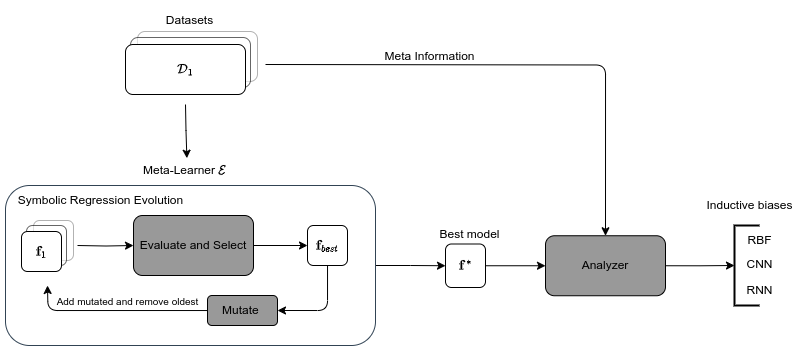
\includegraphics[width=1\textwidth]{model.png}
\end{figure}
Мета-алгоритм \(\mathcal{E}\) принимает на вход наборы данных и эволюционным путем строит модель. Далее лучший кандидат анализируется и делается вывод об индуктивном смещении.
\end{frame}
%----------------------------------------------------------------------------------------------------------
\begin{frame}{Постановка задачи}
Пусть \(\mathfrak{T} = \{T_i\}_{i=1}^n\)~-- множество задач. Каждой задаче \(T_i\) соответствует набор данных \( \mathfrak{D}_i = \{(\mathbf{x}_j, \mathbf{y}_j) \}_{j=1}^{N_i} \). Также обозначим \(\mathfrak{D} = \{ \mathfrak{D}_i\}_{i=1}^n\) и \(\mathfrak{F}\)~-- множество всех моделей.
\begin{itemize}
    \item Моделью \(\mathbf{f}\) назовем отображение из \(X \rightarrow Y\), структура \(\Gamma\) модели которой представима в виде дерева разбора символьного выражения. 
    \item Параметрическим множеством декомпозируемых моделей \(\mathfrak{F}\) назовем множество моделей с одинаковой структурой, которые представимы в виде \(\mathbf{f} = \mathbf{g} \circ \mathbf{h}\). 
    \item Назовем \textit{индуктивным смещением} для декомпозируемой модели структуру первой части \(\mathbf{h}\) модели \(\mathbf{f}\).
    \item Имея функцию потерь задачи \(\mathcal{L}_{\text{task}}\), мы хотим найти индуктивное смещение для декомпозируемой модели по заданному набору выборок:
    \[
        \Gamma = \argmin_{\mathbf{f} = \mathbf{g} \circ \mathbf{h}} \mathbb{E}_{\mathbf{X}, \mathbf{Y}} \mathcal{L}_{\text{task}} (\mathbf{f}(\mathbf{X}), \mathbf{Y})
    \]
\end{itemize}

\end{frame}
%----------------------------------------------------------------------------------------------------------
\begin{frame}{Данные для эксперимента}
Эксперимент проводился на двух задачах:
\begin{enumerate}
    \item \textbf{Бинарная классификация по окружности}: разделение точек, граница классов которых представляет собой окружность. Оптимальной моделью является \textit{кривая второго порядка}.
    \item \textbf{Авторегрессия}: предсказание временного ряда, сгенерированного и использованием авторегрессионной модели. Оптимальная модель находит \textit{временные зависимости}.
\end{enumerate}


\textbf{Гипотеза:} символьное представление модели будет содержать операции характерные для типа задачи.
\end{frame}
%----------------------------------------------------------------------------------------------------------
\begin{frame}{Результаты эксперимента}
\begin{table}
    \footnotesize
    \centering
    \begin{tabular}{|c|c|c|}
        \hline
        \thead{Выборка} & \thead{Кол-во \\ выборок} & \thead{Модели} \\
        \hline
         \multirow{4}{5.5em}{Окружности} & 1 & \(g(x) = x + c_1, \; h(x, y) = (x + c_2)^2 + (y + c_3)^2\) \\
         & 2 & \(g(x) = x + c_1, \; h(x, y) = (x + c_2)^2 + (y + c_3)^2\) \\
         & 5 & \(g(x) = x + c_1, \; h(x, y) = \frac{xy(x + c_2)(x - y)}{c_3 - y}\) \\ 
         & 10 & \(g(x) = \frac{c_1}{x} + c_2, \; h(x, y) = \frac{y}{xc_3} - (x+c_4)(y+c_5)\) \\
         \hline
         \multirow{4}{6.3em}{Авторегрессия} & 1 & \(cx_{t}\) \\
         & 2 & \(cx_{t}\) \\
         & 5 & \(cx_{t}\) \\ 
         & 10 & \(csin^2(x_{t})x_t\) \\
         \hline
    \end{tabular}
    \caption*{Модели для разных размеров выборок.}
    \label{tab:my_label}
\end{table}


\end{frame}
%----------------------------------------------------------------------------------------------------------
\begin{frame}{Вывод}
\textbf{Заключение}:
\small
\begin{itemize}
    \setlength\itemsep{-0.1em}
    \item Предложен метод автоматического определения индуктивного смещения в моделях. 
    \item Проведены предварительные эксперименты на ряде синтетических выборок различного типа.
    \item Эксперименты показали применимость метода.
    % \item 
\end{itemize}
\normalsize \textbf{Дальнейшие исследования}: 
\small 
\begin{itemize}
    \setlength\itemsep{-0.1em}

    \item \textbf{Бинарная классификация цифр (MNIST)}: выявление формулы с ограниченным числом параметров, в которой можно выделить компоненты, аналогичные свёрточными операциями
    \item Интеграция Informational Bottleneck для нахождения оптимальных (в смысле информации) моделей. 
\end{itemize}
\end{frame}
%----------------------------------------------------------------------------------------------------------
% \begin{frame}{Дальнейшие исследования}
% \begin{itemize}
%     \item \textbf{Бинарная классификация цифр (MNIST)}: выявление формулы с ограниченным числом параметров, в которой можно выделить компоненты, аналогичные свёрточными операциями
%     \item Интеграция Informational Bottleneck для нахождения оптимальных (в смысле информации) моделей. 
% \end{itemize}
% \end{frame}
%----------------------------------------------------------------------------------------------------------
\begin{frame}{Источники}
    % \citep{automl-zero}
    \nocite{automl-zero}
    \nocite{Cranmer2023InterpretableML}
    \nocite{symb_ib_dl}
    \nocite{bazarova_structure}
    \bibliographystyle{plain}
    \bibliography{ib_in_model_selection}
    
\end{frame}
%-----------------------------------------------------------------------------------------------------


\end{document} 
